%%=============================================================================
%% Inleiding
%%=============================================================================

\chapter{Inleiding}
\label{ch:inleiding}

%%De inleiding moet de lezer alle nodige informatie verschaffen om het onderwerp te begrijpen zonder nog externe werken te moeten raadplegen \autocite{Pollefliet2011}. Dit is een doorlopende tekst die gebaseerd is op al wat je over het onderwerp gelezen hebt (literatuuronderzoek).

%%Je verwijst bij elke bewering die je doet, vakterm die je introduceert, enz. naar je bronnen. In \LaTeX{} kan dat met het commando \texttt{$\backslash${textcite\{\}}} of \texttt{$\backslash${autocite\{\}}}. Als argument van het commando geef je de ``sleutel'' van een ``record'' in een bibliografische databank in het Bib\TeX{}-formaat (een tekstbestand). Als je expliciet naar de auteur verwijst in de zin, gebruik je \texttt{$\backslash${}textcite\{\}}.
%%Soms wil je de auteur niet expliciet vernoemen, dan gebruik je \texttt{$\backslash${}autocite\{\}}. Hieronder een voorbeeld van elk.

%%\textcite{Knuth1998} schreef een van de standaardwerken over sorteer- en zoekalgoritmen. Experten zijn het erover eens dat cloud computing een interessante opportuniteit vormen, zowel voor gebruikers als voor dienstverleners op vlak van informatietechnologie~\autocite{Creeger2009}.

Voor 22 februari 2017 kon men enkel Docker installeren op Linux-besturingssystemen. Ondernemingen zonder Linux-kennis die wilden evolueren naar DevOps werden op die manier gedwongen om iemand in dienst te nemen die deze kennis wel had, ofwel om zelf een spoedcursus te volgen. Echter met de komst van Windows 10 en Windows Server 2016, en de daarmee gepaard gaande groei van PowerShell en Hyper-V, is Docker nu ook toegankelijk voor organisaties die meer Windows-gezind willen zijn.

Het zou namelijk een vergissing zijn om Docker zomaar te negeren als men de DevOpsrichting wil uitgaan. Het biedt immers verschillende tools aan voor zowel developers als system administrators. Bijvoorbeeld: Containers as a Service (CaaS) en role-based access control voor Operations (system administrators), en een zelfbedieningsmanier van werken voor Developers waarbij ze services kunnen opvragen wanneer ze die nodig hebben. Momenteel wordt Docker gebruikt in 44 procent van de ondernemingen die van plan zijn om de DevOps-richting uit te gaan.

\section{Stand van zaken}
\label{sec:stand-van-zaken}

%% TODO: deze sectie (die je kan opsplitsen in verschillende secties) bevat je
%% literatuurstudie. Vergeet niet telkens je bronnen te vermelden!
\subsection{DevOps}
\label{sec:devops-uitleg}
DevOps is een samenstelling van de woorden ’Development’ en ’Operations’: ontwikkeling en beheer. Voorheen werkten deze IT-groeperingen strikt gescheiden, waardoor je ofwel bij de ene groep zat ofwel bij de andere. Dit zorgde ervoor dat, als men een applicatie wou maken, de developers deze dan eerst ontwikkelden, waarna de systeembeheerders de applicatie uitrolden. Als de systeembeheerders hierna nog problemen hadden met het uitrollen, verliep de communicatie veelal stroef. De applicatie werkte immers op de computers van de developers, dus waarom zou dat niet het geval zijn bij de systeembeheerders? Echter, aangezien beide groeperingen onvoldoende kennis hadden over elkaars werkveld, was er veel onbegrip.

\begin{figure}
	\caption{Links ziet men hoe de communicatie in klassieke ontwikkelomgevingen gebeurt, rechts in DevOps teams}
	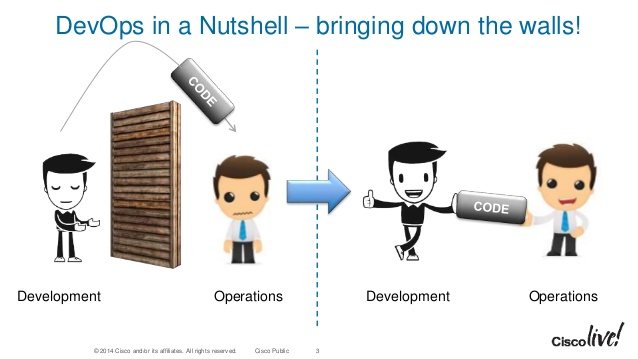
\includegraphics[scale=0.6]{img/devopsmuur.jpg}
	\label{fig:devopsmuren}
\end{figure}

Als éénduidige definitie voor DevOps gebruikt met het acroniem 'CALMS'.
\begin{itemize}[noitemsep]
	\item Culture (Cultuur)
	\item Automatisation (Automatisatie)
	\item Learning (Leren, voorheen Lean)
	\item Measure (Meten)
	\item Sharing (Delen)
\end{itemize}

Bij DevOps worden deze groepen gedwongen om samen te werken in één team, zodat het geheel groter wordt dan de som. In praktijk vertaalt dit zich naar een cultuur die gestimuleerd dient te worden, waarin het automatiseren van zoveel mogelijk zaken centraal staat met een focus op continue ontwikkeling en oplevering (cfr. CI/CD). Hierbij is het leren, delen van informatie, en communicatie in het algemeen, heel belangrijk. Er worden verschillende manieren voorzien om informatie te verzamelen uit de applicatie, door methodes te implementeren die men gebruikt om een doorzichtiger systeem te creëren. Het is dus eerder een groep van concepten en ideeën die uitgegroeid zijn tot een beweging die snel tractie aan het winnen is.

\begin{center}
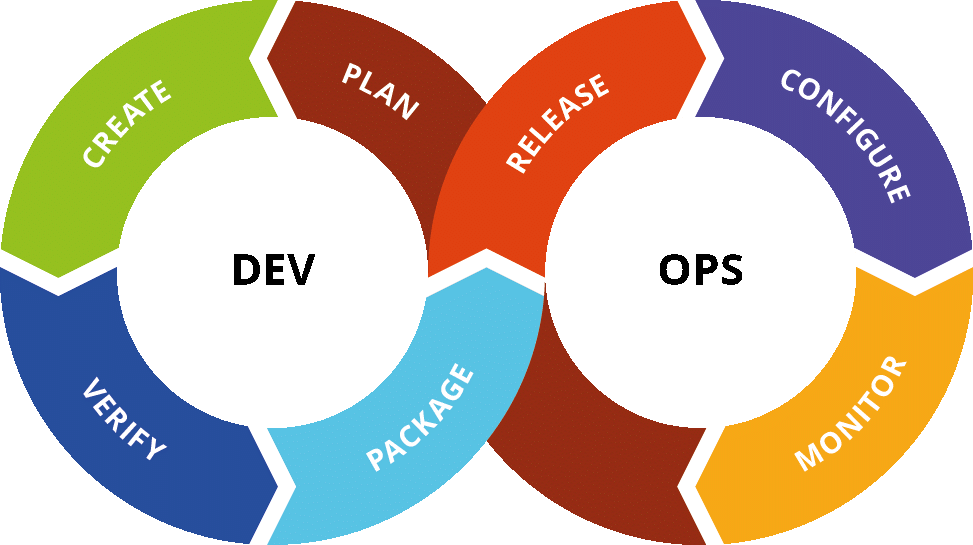
\includegraphics[scale=0.5]{img/devops.png}
\end{center}

\subsection{Docker}
\label{sec:docker-uitleg}
De beste manier om de verschillen in werking te beschrijven tussen fysieke servers, virtuele machines (VM’s) en containers, is door ernaar te kijken zoals een woning. Fysieke servers en virtuele machines zijn zoals huizen. Ze werken volledig onafhankelijk en voorzien zelf in al hun noden qua infrastructuur. Een fysieke server wordt bovendien volledig onafhankelijk opgebouwd vanaf nul. Een virtuele machine echter wordt naast een bestaand host besturingssysteem gedraaid, waarbij het een bepaalde hoeveelheid infrastructuur opeist. Een virtuele machine is dus eigenlijk een computer in een computer. Beide systemen hebben hetzelfde grote nadeel, namelijk dat er veel meer infrastructuur nodig is en dat deze niet optimaal wordt gebruikt. Containers zijn eerder te vergelijken met appartementen, namelijk dat de infrastructuur wordt opgedeeld. Alle middelen van de host-machine waar de Docker Daemon op geïnstalleerd wordt, worden verdeeld onder de verschillende containers. Elke container vraagt hierbij alleen de nodige grondstoffen om te voldoen aan de noden van zijn bewoner, net zoals bij een appartement. Containers lijken op het eerste zicht erg op virtuele machines, maar het is belangrijk om te onthouden dat de onderliggende architectuur sterk verschilt tussen beide.

Doordat een Container alleen de benodigde infrastructuur opeist die hij nodig heeft, bouwt die een lichter en onafhankelijk uitvoerbaar softwarepakket op, dat consistentie kan garanderen omdat het telkens dezelfde achterliggende Docker Images en Daemon gebruikt. Een van de meest voorkomende problemen bij het uitrollen van een applicatie is het verschil tussen de test- en productieomgeving, en de hiermee gepaarde infrastructuurlast.

\begin{center}
	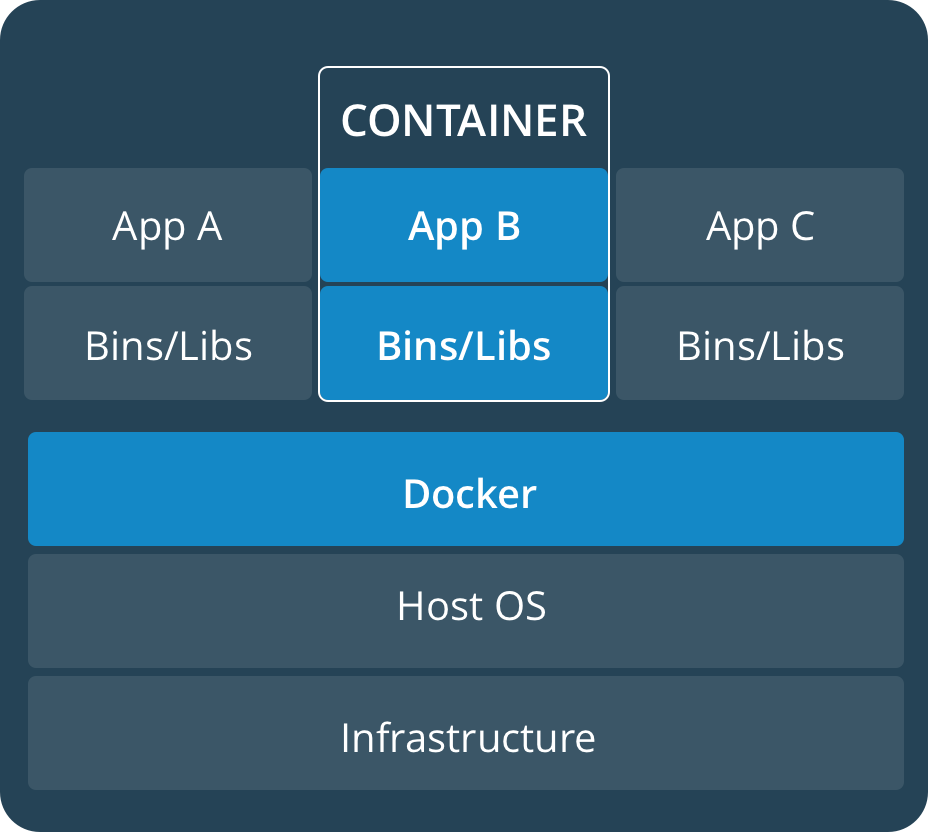
\includegraphics[scale=0.2]{img/containers.png}
	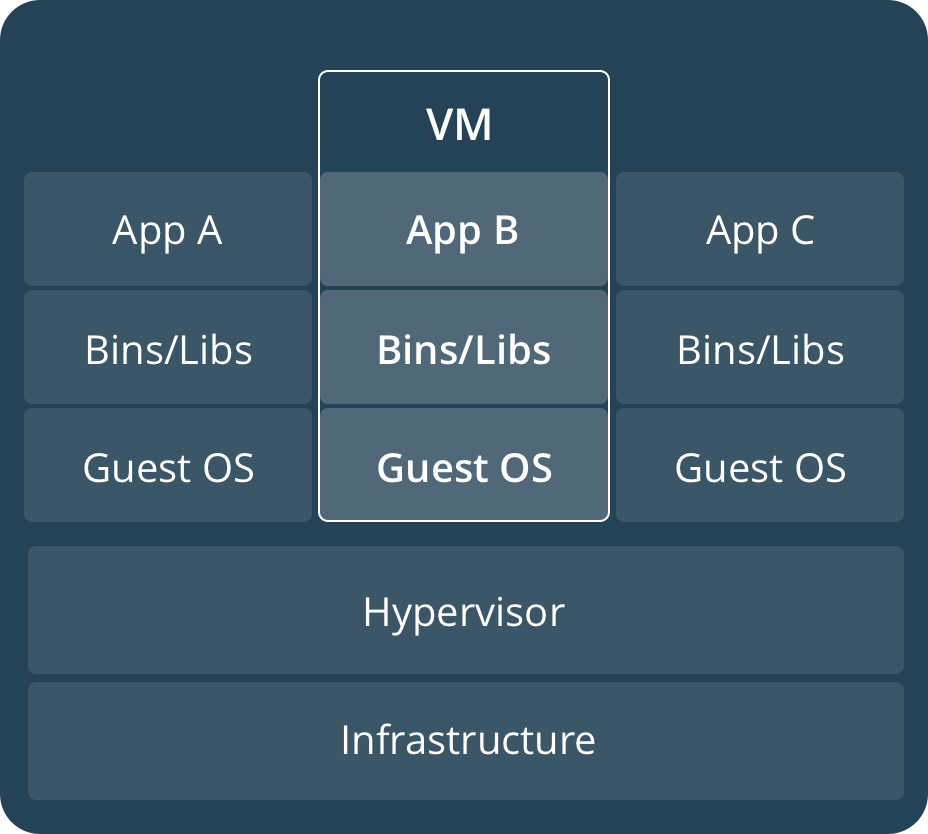
\includegraphics[scale=0.2]{img/vms.png}
\end{center}

Docker is een tool om deze Containers te bouwen. Hiermee kan men het uitrollen van applicaties sneller en makkelijker maken, doordat het de applicatie en al haar benodigdheden eerst in één geautomatiseerd pakket verzamelt. Dit pakket noemt een image. De uitgerolde versie van een image noemt men een Container en deze zal los van het host besturingssysteem werken.

Om een Container op te bouwen van begin tot einde maakt men gebruik van de Docker Client. Via de Client kan men communiceren met de Docker Daemon. De Docker Daemon is een proces dat op de achtergrond draait tot het aangeroepen wordt door de gebruiker via de syntaxis van Docker. De Docker Daemon is uiteindelijk degene die de Docker commando's interpreteert en uitvoert, zoals het bouwen, draaien en onderhouden van containers.

Bij het bouwen van een container via Docker zijn er 23 werkmethodes te onderscheiden, namelijk een standaard-, minimalistische- of geautomatiseerde methode. De minimalistische methode wordt gebruikt bij installaties die geen customisation vereisen, bijvoorbeeld een SQL-server. De standaardmethode wordt gebruikt bij alle andere installaties, bijvoorbeeld een CentOS-server. De standaardmethode bestaat uit 4 stappen die hieronder meer uitgebreid besproken worden. Bij de minimalistische methode worden enkel de eerste en de laatste stap uitgevoerd.

\begin{itemize}[noitemsep]
	\item docker pull
\end{itemize}
De eerste stap is docker pull. Hiermee kan men een Docker Image ophalen van de Docker Hub. Deze images zijn momentopnames van bijvoorbeeld containers of besturingssystemen. Deze kunnen, afhankelijk van de gebruiker, uitgebreid worden via een Dockerfile. Het is met deze parent image dat men een container kan bouwen.

\begin{itemize}[noitemsep]
	\item Dockerfile
\end{itemize}
De tweede stap is Dockerfile, waarin men aan de hand van de syntaxis een gepersonaliseerde Docker Image kan definiëren. Men kan aangeven vanaf welke image men wil beginnen via het 'FROM'-commando. Men hoeft hier echter niet per se een parent image mee te geven, bijvoorbeeld via 'FROM scratch'. Vervolgens kan men environment variables meegeven via 'ENV', 'ADD' of 'EXPOSE'. Daarnaast kan men via 'RUN' ook orders meegeven om specifieke commando's uit te voeren die de container zou herkennen zoals Bash of PowerShell. Ten slotte kan men via 'ENTRYPOINT' aangeven of de container uitvoerbaar moet zijn of niet.

\begin{itemize}[noitemsep]
	\item docker build
\end{itemize}
De derde stap is docker build, waarmee men opnieuw de Docker Daemon aanspreekt. Op die manier kan die de syntaxis interpreteren en een gepersonaliseerde container bouwen.

\begin{itemize}[noitemsep]
	\item docker run <options> <image>
\end{itemize}
Ten slotte is er docker run, waarmee men het bevel geeft aan de Docker Daemon om de image uit te rollen tot een container. Hoe de image zich uitrolt, hangt af van de bevelen in het commando en van de image die gebruikt wordt. 

Bij de geautomatiseerde methode maakt men ook gebruik van de 4 hierboven beschreven stappen. Maar, voegt men een extra component toe in de vorm van docker-compose.yml. In dit bestand kan men meerdere services beschrijven waarvan Docker containers moet maken. Daarnaast dient dit bestand geplaatst te worden in dezelfde folder als het 'dockerfile'-bestand. Ten slotte, zullen alle services die hierin beschreven staan in orde gebracht worden door het 'docker-compose up'-commando uit te voeren.

Docker-compose is daarom vooral handig wanneer men meerdere services wil in orde brengen die afhankelijk zijn van elkaar, zoals een webapplicatie en de bijhorende SQL-server. Hieronder ziet u een voorbeeld van een docker-compose.yml-bestand.

backend: 
	image: redis:3 
	restart: always

frontend: 
	build: commander 
	links: 
		- backend:redis  
	ports: 
		- 8081:8081 
	environment: 
		- VAR1=value 
	restart: always

Docker voorziet ook commando's om de Docker Images en Boxes te beheren. De voornaamste staan hieronder beschreven.

\begin{tabular}{ll}
	\hline
	Commando & Uitleg \\
	\hline
	docker images & toont alle Docker Images beschikbaar op dit systeem \\
	docker ps & toont alle draaiende containers \\
	docker inspect <container> & toont de specificaties van een specifieke container \\
	docker logs <container> & toont alle logs voor een specifieke container \\
	docker start <container> & start een specifieke container op \\
	docker stop <container> & stopt een specifieke container \\
	docker rm <container> & verwijdert containers \\
	\hline
\end{tabular}

Doordat elk deel van een applicatie in een 'appartementje' zit, is het maken van continue ontwikkeling en oplevering voor de applicatie heel gemakkelijk. Men moet immers alleen die specifieke Container updaten/graden. Hierdoor is het de perfecte technologie om te dienen als test- en productieomgeving. Daarnaast versoepelt het ook de communicatie binnen het DevOps-team, doordat iedereen continu in dezelfde omgeving werkt. Er zijn immers geen grote veranderingen nodig bij de verschillende stappen binnen de leveringsketen, omdat men in staat is om verschillende frameworks te draaien op één platform. Containers zijn namelijk vrij agnostisch zijn op vlak van programmeertaal of platform. Ten slotte kunnen Containers ook makkelijk van host-besturingssysteem verplaatst worden. Al deze kenmerken van Docker Containers vergemakkelijken het werk van DevOps-teams aanzienlijk.

Door al deze redenen blijft Docker ook jaar na jaar groeien. Tijdens de recentste DockerCon heeft de CEO van Docker dit ook aangetoond met volgend cijfermateriaal:
\begin{itemize}[noitemsep]
	\item Meer dan 14 miljoen Docker hosts
	\item More dan 900.000 applicaties die draaien op Docker
	\item Een verhoging van 40 procent in het toepassen ervan in 1 jaar
\end{itemize}

Docker heeft deze groei ook verdiend door constant in contact te blijven met zijn gebruikers. In het verleden kregen ze immers de klacht dat ze te snel of te traag updates toevoegden aan het systeem. Om dit te remediëren hebben ze naast Docker Community Edition, waarmee alles is begonnen, nu ook Docker Enterprise Edition ontworpen. Daarbovenop is er een verschuiving naar time-based updates. Hierbij kan men kiezen tussen een maandelijkse update, maar zonder garantie op stabiliteit van de runtime (Edge), ofwel voor een viermaandelijkse update voor gebruikers die meer stabiliteit prefereren, zowel op vlak van onderhoud als van beheer (Stable). Daarbovenop heeft de Enterprise Edition ook een meer uitgebreide ondersteuning met verschillende gradaties.

\subsubsection{Docker CE}
Zoals eerder aangehaald is Docker Community Edition het originele platform waarmee Docker begonnen is. Het is ideaal voor kleinere teams of onafhankelijke developers die willen experimenteren met Container-technologie. Deze technologie is beschikbaar voor zowel Linux als Mac, waardoor het perfect is als kleine en snelle installatie waarmee men direct aan de slag kan gaan. Ten slotte, biedt het ook ondersteuning voor het uitrollen naar Cloud-omgevingen, zoals Amazone Web Services of Azure. 

\subsubsection{Docker EE}
Docker Enterprise Edition is het volledige pakket voor zij die op een professionele manier met een Containers-as-a-Serivce-platform willen werken. Docker EE is een geïntegreerd en getest platform voor Linux- of Windows Enterprise en Cloud-providers, met door Docker gecertificeerde componenten en ondersteuning. In het bijzonder is het voor datacenters een handig dashboard waar men de zogenaamde multi-architecture orchestration, secure software supply chain en infrastructure independence aangeboden krijgt. Vooral aan dat laatste heeft Docker extra veel aandacht besteed., met kenmerken zoals trusted delivery.

\subsubsection{Docker for Windows}
Daarnaast heeft Docker ook een versie ontwikkeld specifiek gericht voor Developers die gebruik willen maken van Windows als ontwikkel platform. Docker for Windows maakt gebruik van dezelfde Daemon en Client als Docker for Linux. Maar, met een paar verschillen zoals: Docker for Windows maakt gebruik van de Windows-native Hyper-V Virtualisatie. Wat betekent dat de gebruiker een Windows 8+ Pro edition of een Windows Server 2008+ nodig heeft. Aangezien alleen deze versies van Windows Hyper-V hebben. Daarnaast is de enige manier om Docker CE for Windows te installeren door gebruik te maken van een GUI installatie. Men kan gebruik maken van PowerShell commando's zoals Invoke-Webrequest. Maar, er is geen native PowerShell commando voor het installeren van Docker for Windows. Docker EE for Windows kan dan weer wel via de commandline geinstalleerd worden. Ten slotte, wordt docker-compose ook automatisch geïnstalleerd als men Docker CE for Windows installeert. Het maakt deel uit van het totaal pakket. Dit in tegenstelling tot Docker EE for Windows, waarbij docker-compose wél nog apart geïnstalleerd moet worden.

\begin{center}
	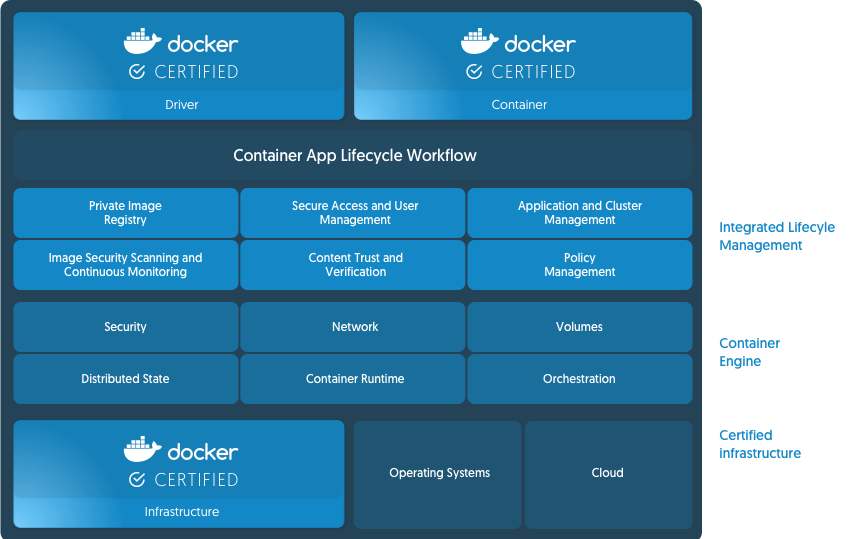
\includegraphics[scale=0.2]{img/dockerce.png}
\end{center}

\subsection{Linux Containers}
Docker CE for Linux maakt gebruik van de technologie achter Linux Container voor het maken van zijn Docker Containers.

Linux containers hebben hun eigen netwerk resources, geheugen geïsoleerde CPU, geheugen en I/O block. Maar, ze gebruiken wel dezelfde kernel als het host besturingssysteem. Hierdoor kunnen ze lichte en gestroomlijnde containers bouwen. Cgroups en Namespaces maakt dit mogelijk.

\subsubsection{Cgroups}


\subsubsection{Namespaces}


\subsection{Hyper-V}
Hyper-V is één van de technologie die gekozen werd om de twee servers, CentOS en Windows Server 2016, op te laten draaien. Dit is het Microsoft-platform voor het virtualiseren van hardware. Het maakt gebruik van hypervisor-gebaseerde virtualisatie technologie om de interactie tussen de virtuele machine en de hardware te voorzien. Hierdoor is men in staat om een andere computer te laten werken bovenop het host-besturingssysteem. De voornaamste componenten en hun functies van dit platform zijn:

\begin{itemize}[noitemsep]
	\item Windows Hypercall
\end{itemize}

Hypercall voorziet communicatie met de Hypervisor.

\begin{itemize}[noitemsep]
	\item Windows hypervisor
\end{itemize}

Dit is een softwarelaag wiens primaire verantwoordelijkheid is om geïsoleerde execution enviroments te voorzien. Deze execution enviroments noemen partitions. Hypervisor is gelegen tussen de hardware en één of meer besturingssystemen, zodat het hardwaregebruik kan optimaliseren voor al de partitions.

\begin{itemize}[noitemsep]
	\item Hyper-V Virtual Machine Management Service
\end{itemize}

VMMS is verantwoordelijk voor het beheren van de staat van alle virtuele machines in zogenaamde child partitions.

\begin{itemize}[noitemsep]
	\item Virtual Machine Bus
\end{itemize}

Dit channel-based communicatiemechanisme voorziet de communicatie tussen verschillende partitions op systemen met meer dan één virtual partition.

\begin{itemize}[noitemsep]
	\item Virtualization Service Provider
\end{itemize}

VSP bevindt zich in de root partition en voorziet synthetische ondersteuning aan child partitions over de VMBus.

\begin{itemize}[noitemsep]
	\item Virtual Infrastructure Driver
\end{itemize}

De VID voorziet partition-, processor- en memory services.

Daarnaast bevat Hyper-V ook nog andere low level componenten, zoals:

\begin{itemize}[noitemsep]
	\item APIC - Advanced Programmable Interrupt Controller
	\item IC - Integration component
	\item MSR - Memory Service Routine
	\item VMWP - Virtual Machine Worker Process 
	\item VSC - Virtualization Service Client
	\item WinHv  - Windows Hypervisor Interface Library 
	\item WMI - Virtual Machine Management Service 
\end{itemize}

Tenslotte heeft Hyper-V ook enkele tools voor het beheren van en verbinden met zijn virtuele machines. Deze kunnen geïnstalleerd worden op zowel computers waar Hyper-V op staat, als op externe computers. Deze zijn meer specifiek:

\begin{itemize}[noitemsep]
	\item Hyper-V Manager
	\item Hyper-V module for Windows PowerShell
	\item Virtual Machine Connection
	\item Windows PowerShell Direct
\end{itemize}

Om deze servers te verbinden met het internet wordt ook gebruik gemaakt van de Hyper-V Virtual Switch. Deze laag 2 Ethernet netwerkswitch voorziet programmeer- en uitbreidbare mogelijkheden om het beheren van virtuele en fysieke netwerken te vergemakkelijken. Het voorziet veiligheid, isolatie en service levels om de nodige veiligheid af te dwingen.

Hyper-V is een type 1 Hypervisor. Dit betekent dat het opstarten van een virtuele machine als volgt gaat:
\begin{itemize}[noitemsep]
	\item Eerst wordt de fysieke machine opgestart.
	\item Vervolgens wordt de controle van het boot systeem van de fysieke machine overgedragen aan Hyper-V, bijvoorbeeld BIOS of EUFI.
	\item Daarna start Hyper-V het management operating system.
	\item Ten slotte maakt Hyper-V partitions aan voor de virtuele machines, afhankelijk van de boot- of gebruikersinstructies.
\end{itemize}
Daarnaast draait een type 1 Hypervisor ook direct op de hardware. Daarom worden ze ook wel 'native', 'bare metal' of 'embedded' Hypervisors genoemd.

\subsection{Windows Job objects}
=cgroups
process grouping en resource controls

\subsection{Silos}
= namespaces
isolation execution environment voor file system, geistry en object namespaces.

\subsection{Virtual Box}
Virtual Box is de tweede Hypervisor die ondersteund wordt in deze bachelorproef. Deze wordt ontwikkeld door Oracle Corporation, maar is wel een type 2 Hypervisor. Type 2 Hypervisors gedragen zich meer als een gewone software applicatie en worden daarom 'host' Hypervisors genoemd. Ze maken een abstractie van de verbinding met de hardware en moeten hiervoor requests sturen naar het host OS, net zoals gewone applicaties.

De opstartvolgorde is hierdoor ook anders:
\begin{itemize}[noitemsep]
	\item Eerst wordt de fysieke machine gestart.
	\item Vervolgens wordt de controle van het boot systeem van de fysieke machine overgedragen aan Virtual Box, bijvoorbeeld BIOS of EUFI.
	\item Daarna start een gebruiker de Virtual Box applicatie op.
	\item Ten slotte zal de gebruiker kiezen welke virtuele machines worden opgestart, waarbij Virtual Box de benodigde hosting processes aanmaakt.
\end{itemize}

Ten slotte bestaat Virtual Box uit een soortgelijke lijst van componenten, waarbij er toch kleine wijzigingen zijn omdat het een type 2 is.
\begin{itemize}[noitemsep]
	\item IPRT (a portable runtime library)
	\item Virtual Machine Monitor
	\item Execution Manager
	\item Recompiled Execution Monitor
	\item Trap Manager
	\item Hardware Acceleration Manager
	\item Guest Interface Manager
	\item Pluggable Device Manager
	\item Page Manager
	\item Patch Manager
	\item Time Manager
	\item Configuration Manager
	\item Saved State Manager
	\item Virtual USB
	\item Debug Facility
\end{itemize}

\subsection{Vagrant}
Vagrant is een tool voor het bouwen en onderhouden van virtuele machines. Het maakt gebruik van een enkele workflow voor het automatiseren van ontwikkelomgevingen. Doordat het zo makkelijk te gebruiken is, verlaagt het de installatietijd en verhoogt het de productie. Dit is waarom het een geliefde tool is binnen DevOps-teams.

Vagrant werkt aan de hand van een configuratiebestand dat uitgelezen moet worden. Dit configuratiebestand dat Vagrant nodig heeft, heet een 'Vagrantfile'. Hierin wordt alles gedefinieerd dat nodig is, meer bepaald: welke box, scripts en andere bestanden er nog nodig zijn voor de installatie.

Een 'Vagrant Box' is een verpakte base image die een clone is van een virtuele machine. Een base image is het minimum van een besturingssysteem waarop er nog verschillende andere functies gebouwd kunnen worden, zoals bijvoorbeeld een GUI. Via deze box wordt een besturingssysteem en bijbehorende software geïnstalleerd. Deze boxes worden opgehaald door middel van 'config.vm.box = boxnaam'. Als de box nog niet eerder gebruikt werd, wordt deze eerst gedownload vanop Vagrant Cloud, waarna de box wordt opgeslagen zodat deze steeds beschikbaar is voor later gebruik.

Als de box goed is, maar er moet nog verdere installatie of configuratie van de software gebeuren, kan men deze ook meegeven met het 'provision'-gedeelte. Met provisioning voegt men verdere configuratiemogelijkheden toe, zoals het uitvoeren van scripts, het uploaden van bestanden of folders tijdens de installatie, of het specificeren van een netwerkadres. Door provisioning kan men ook makkelijk wijzigingen aanbrengen aan het systeem tijdens de run-time. Er wordt ook gebruik gemaakt van een eigen syntax die aangeleerd dient te worden. Deze bestaat uit 'vagrant' en de functie die uitgevoerd dient te worden, bijvoorbeeld: met 'vagrant up' wordt geprobeerd om het systeem online te brengen. De configuratie van de 'Vagrantfile' heeft ook zijn eigen syntax, bestaande uit het woord ’config’ en de functie bepalend wat ermee moet gebeuren.

Vagrant ondersteunt bovendien verschillende platformen om zijn installatie op uit te voeren, gaande van VirtualBox en Hyper-V tot Docker en AWS. Het grote aantal beschikbare platformen om op te releasen is ook een sterkte van Vagrant.

Daarbovenop zijn er mogelijkheden om de functionaliteit van Vagrant zelf uit te breiden door gebruik te maken van plug-ins die geschreven worden door andere gebruikers, of door gebruik te maken van andere Configuration Management tools, zoals Ansible. Plug-ins worden meestal geschreven in de programmeertaal Ruby. Voor de gebruikte Windows Server-opstelling in deze bachelorproef is deze functionaliteit heel handig, omdat de Windows Server herstart dient te worden na de installatie van Docker. Hiervoor kan een plug-in gebruikt worden.

Om al deze redenen werd geopteerd om gebruik te maken van deze technologie. Er zijn gelijkaardige zero-touch installatiemogelijkheden, zoals Chef, Puppet of Terraform. Echter geen van hen biedt hetzelfde gebruiksgemak of dezelfde mogelijkheden.

\subsection{PowerShell}
De configuratie van de Windows Server gebeurt grotendeels aan de hand van deze command-line inteface. Deze CLI, die bovendien gebruik maakt van het .NET framework om objecten terug te geven, is namelijk speciaal ontwikkeld voor system administrators. Een groot voordeel hierbij is dat objecten veel makkelijker te verwerken zijn, in tegenstelling tot andere CLI’s die vaak tekst gebruiken voor het uitvoeren van commando’s. Daarnaast is de structuur van de command-lets (cmdlet) simpel en makkelijk aan te leren. De commando’s bestaan namelijk altijd uit dezelfde samenstelling, bestaande uit 'werkwoord'-'te behandelen onderwerp', bijvoorbeeld: Get-Service.

\subsection{Bash}
Als tegenpool is er Bash voor Linux besturingssystemen. Deze CLI dateert al van 1989, met als volledige naam 'Bourne Again shell'. In essentie werkt Bash op dezelfde wijze als PowerShell. Net zoals PowerShell herkent Bash namelijk een aantal woorden, waardoor men ermee kan communiceren en het acties kan laten uitvoeren. Het grote verschil ligt in de uitvoering: Bash heeft namelijk enkel tekst als in- en uitvoer, wat het verwerken van opdrachten kan bemoeilijken. Echter, omdat Bash reeds geruime tijd bestaat, kan deze Unix shell wel genieten van een enorme gebruiks- en ondersteuningsbasis. Bash is namelijk de werkmethode bij uitstek voor Linux administrators.

%% Lagen software testing uitleggen
%% Beter verwoorden
%% Meer

\subsection{Software testing}
\label{sec:testing-uitleg}
Bij software testing ligt de focus op kwaliteit in alle delen van de organisatie. Dit is belangrijk omdat het ontwikkelingsteam verantwoordelijk is voor de kwaliteit. QA-teams kunnen op tijd aan de alarmbel trekken, maar de verantwoordelijkheid van kwaliteit ligt nog steeds bij het ontwikkelingsproces. Daarom eist software testing dat iedereen, inclusief de gebruiker, betrokken is bij het ontwikkelingsproces. Software testing heeft een methodologische manier ontwikkeld om de kwaliteit te waarborgen, waarbij men laag per laag en stap per stap gaat kijken of het systeem voldoet aan de vereisten.

\begin{center}
	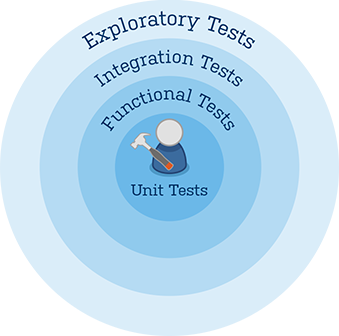
\includegraphics[scale=0.5]{img/testing.png}
\end{center}

Verder zegt REF over software testing dat het een empirische en technische manier is om software of services te testen, doordat men op een objectieve manier kijkt naar de kwaliteit van een software of service. Dit is de voornaamste reden waarom voor deze methode gekozen is in deze bachelorproef. Daarnaast sluit het heel goed aan bij de principes van het DevOps manifesto.

Meer specifiek wordt er gebruik gemaakt worden van performantie- en veiligheidstesten.

Performantietesten zijn testen waarbij men gaat kijken hoe het systeem presteert wanneer het een bepaalde werkdruk moet verwerken, met de focus op snelheid, schaalbaarheid en stabiliteit.

Bij veiligheidstesten wordt er gekeken naar alle verschillende veiligheidsmaatregelen, en in hoeverre ze in staat zijn om de zwaktes van het systeem te beschermen.

\begin{center}
	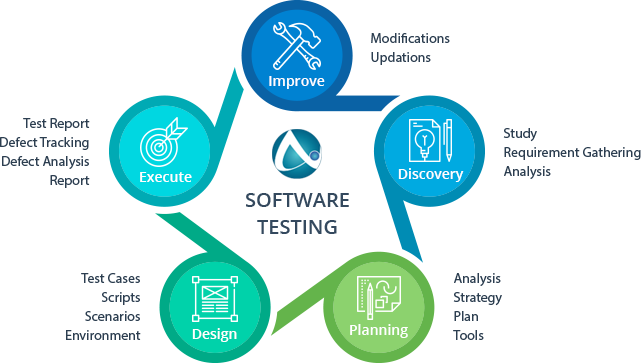
\includegraphics[scale=0.5]{img/testingprocess.png}
\end{center}

\section{Probleemstelling en Onderzoeksvragen}
\label{sec:onderzoeksvragen}

%% TODO:
%% Uit je probleemstelling moet duidelijk zijn dat je onderzoek een meerwaarde
%% heeft voor een concrete doelgroep (bv. een bedrijf).
%%
%% Wees zo concreet mogelijk bij het formuleren van je
%% onderzoeksvra(a)g(en). Een onderzoeksvraag is trouwens iets waar nog
%% niemand op dit moment een antwoord heeft (voor zover je kan nagaan).

Het grootste probleem bij Docker is dat het op zich nog een relatief jonge technologie is, die bovendien een eigen syntaxis heeft. Daarnaast is er een andere denk- en werkwijze vereist om Docker te beheersen. Doorheen de tijd zijn Linux administrators reeds vertrouwd geraakt met deze technologie, maar voor Windows administrators is deze werkomgeving
nog gloednieuw.

De onderzoeksvragen die uit deze probleemstelling voortvloeien zijn de volgende:

\begin{itemize}[noitemsep]
	\item Hoe vlot kan men een Docker-opstelling maken op een Windows-besturingssysteem tegenover een Linux-besturingssysteem?
	\item Hoe is het gesteld met de documentatie voor Docker for Windows tegenover de bestaande documentatie voor Linux?
	\item Hoe groot is de snelheidswinst bij Linux tegenover Windows?
	\item Hoe is het gesteld met de veiligheid? Hoe pakt men deze aan vanuit een Windows administrator perspectief?
\end{itemize}

Op al deze vragen kon tot op heden geen afdoend antwoord worden gegeven. Men heeft in het verleden wel al Docker for Windows uitgetest en vergeleken met Linux, maar nooit op een concrete en methodische manier. Vaak benaderde men deze technologie ook vanuit een bestaande mening, en niet vanuit een neutraal perspectief.

Dit onderzoek zal vooral een grote meerwaarde zijn voor DevOps-teams die op zoek zijn naar Windows-oplossingen voor hun problemen in verband met automatisatie en continue oplevering.

\section{Opzet van deze bachelorproef}
\label{sec:opzet-bachelorproef}

%% TODO: Het is gebruikelijk aan het einde van de inleiding een overzicht te
%% geven van de opbouw van de rest van de tekst. Deze sectie bevat al een aanzet
%% die je kan aanvullen/aanpassen in functie van je eigen tekst.

De rest van deze bachelorproef is als volgt opgebouwd:

In Hoofdstuk~\ref{ch:methodologie} wordt de methodologie toegelicht en worden de gebruikte onderzoekstechnieken besproken om een antwoord te kunnen formuleren op de onderzoeksvragen.

In Hoofdstuk~\ref{ch:documentatie} wordt de documentatie van beide platformen besproken. Er wordt gekeken naar volledigheid, interne en externe bronnen, en hoeveel ondersteuning er is vanuit de hoofdorganisatie.

In Hoofdstuk~\ref{ch:opstelling} worden beide opstellingen bekeken en besproken, meer specifiek hoe het is om beide op te bouwen, en hoe het zit met gelijkenissen en verschillen.

In Hoofdstuk~\ref{ch:performantietest} wordt gekeken naar het resultaat van de werklading dat beide systeem te verduren hebben gekregen en hoe ze beide gepresteerd hebben.

In Hoofdstuk~\ref{ch:securitytest} worden de beschikbare veiligheidsmaatregelen voor Docker besproken binnen beide systemen en hoe effectief deze zijn.

In  Hoofdstuk~\ref{ch:conclusie} wordt ten slotte een conclusie gevormd en wordt er een antwoord geformuleerd op de onderzoeksvragen. Hierbij wordt ook een aanzet gegeven naar mogelijk toekomstig onderzoek binnen dit domein.

